\chapter{Integrali di Superficie di 2ª Specie}

\section{Definizione e Significato Geometrico}
Gli integrali di superficie di seconda specie si applicano esclusivamente alle \textbf{superfici orientabili}.

La definizione formale è data dall'integrale:
\[
\iint_S \vec{F} \cdot \vec{n} \, dS
\]
Dal punto di vista fisico e geometrico, questa quantità si chiama \textbf{flusso del campo vettoriale $\vec{F}$ attraverso la superficie $S$}.

\begin{figure}[H]
    \centering
    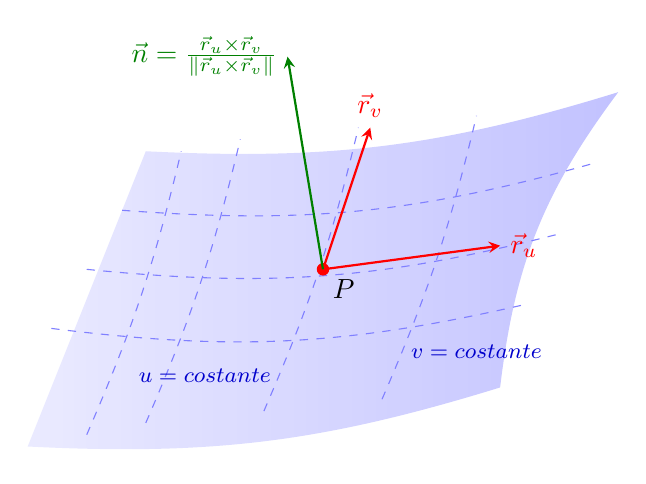
\begin{tikzpicture}[scale=1.5, >=stealth]
        
        % Disegno la superficie curva (patch) in 3D
        \shade[left color=blue!10, right color=blue!30, opacity=0.8] 
            (0,0) to[bend right=10] (4,0.5) to[bend left=15] (5,3) to[bend left=10] (1,2.5) -- cycle;
            
        % Linee di griglia u=costante, v=costante
        \draw[blue!50, thin, dashed] (0.5,0.1) to[bend right=5] (1.3, 2.5);
        \draw[blue!50, thin, dashed] (1.0,0.2) to[bend right=5] (1.8, 2.6);
        \draw[blue!50, thin, dashed] (2.0,0.3) to[bend right=5] (2.8, 2.7);
        \draw[blue!50, thin, dashed] (3.0,0.4) to[bend right=5] (3.8, 2.8);
        
        \draw[blue!50, thin, dashed] (0.2,1.0) to[bend right=10] (4.2, 1.2);
        \draw[blue!50, thin, dashed] (0.5,1.5) to[bend right=10] (4.5, 1.8);
        \draw[blue!50, thin, dashed] (0.8,2.0) to[bend right=10] (4.8, 2.4);

        % Punto P sulla superficie
        \coordinate (P) at (2.5, 1.5);
        \fill[red] (P) circle (1.5pt) node[below right, text=black] {$P$};
        
        % Vettore r_u tangente
        \draw[->, thick, red] (P) -- ++(1.5, 0.2) node[right] {$\vec{r}_u$};
        % Vettore r_v tangente
        \draw[->, thick, red] (P) -- ++(0.4, 1.2) node[above] {$\vec{r}_v$};
        % Vettore normale n (prodotto vettoriale)
        \draw[->, thick, green!50!black] (P) -- ++(-0.3, 1.8) node[left] {$\vec{n} = \frac{\vec{r}_u \times \vec{r}_v}{\|\vec{r}_u \times \vec{r}_v\|}$};

        % Etichette delle curve coordinate
        \node[blue!80!black, font=\footnotesize] at (3.8, 0.8) {$v = \text{costante}$};
        \node[blue!80!black, font=\footnotesize] at (1.5, 0.6) {$u = \text{costante}$};

    \end{tikzpicture}
    \caption{Costruzione del versore normale $\vec{n}$ alla superficie tramite il prodotto vettoriale dei vettori tangenti $\vec{r}_u$ e $\vec{r}_v$.}
\end{figure}

\section{Riduzione a un Integrale Doppio}
Vogliamo ridurre questo integrale di superficie a un classico integrale doppio sul dominio base $D$, in modo da poterlo calcolare in modo esplicito. Come lo possiamo parametrizzare?

Immaginiamo di avere una superficie descritta in forma parametrica tramite le sue curve coordinate. Fissando alternativamente i parametri, otteniamo le curve $u = \text{costante}$ e $v = \text{costante}$.

Per costruzione, i vettori derivati $\vec{r}_u$ e $\vec{r}_v$ sono vettori \textbf{tangenti} alla superficie in un dato punto.
Se facciamo il loro prodotto vettoriale, otterremo un vettore ortogonale alla superficie stessa. Da questo possiamo ricavare il versore normale $\vec{n}$:
\[
\vec{n} = \frac{\vec{r}_u \times \vec{r}_v}{\left\| \vec{r}_u \times \vec{r}_v \right\|}
\]

Sostituendo nell'integrale originale il versore $\vec{n}$ e il differenziale d'area $dS = \left\| \vec{r}_u \times \vec{r}_v \right\| du \, dv$, le norme si elidono perfettamente:

\[
\iint_S \vec{F} \cdot \vec{n} \, dS = \iint_D \vec{F} \cdot \left( \frac{\vec{r}_u \times \vec{r}_v}{\left\| \vec{r}_u \times \vec{r}_v \right\|} \right) \left\| \vec{r}_u \times \vec{r}_v \right\| du \, dv
\]

Otteniamo così la formula risolutiva finale, che rende l'integrale calcolabile:
\[
\iint_S \vec{F} \cdot (\vec{r}_u \times \vec{r}_v) \, du \, dv
\]

\section{Esercizio: Area della superficie sferica}
Calcolare l'area della superficie di una sfera di raggio $R$.

\subsection*{Parametrizzazione}
Scegliamo la seguente parametrizzazione per la superficie sferica utilizzando i parametri $\theta$ e $\rho$:
\[
\vec{r}(\theta, \rho) =
\begin{bmatrix}
R \cos\theta \cos\rho \\
R \cos\theta \sin\rho \\
R \sin\theta
\end{bmatrix}
\]

\subsection{Derivate parziali}
Calcoliamo le derivate parziali del vettore posizione rispetto ai parametri $\theta$ e $\rho$:
\[
\vec{r}_\theta =
\begin{bmatrix}
-R \sin\theta \cos\rho \\
-R \sin\theta \sin\rho \\
R \cos\theta
\end{bmatrix}
\]
\[
\vec{r}_\rho =
\begin{bmatrix}
-R \cos\theta \sin\rho \\
R \cos\theta \cos\rho \\
0
\end{bmatrix}
\]

\subsection{Prodotto vettoriale e vettore normale}
Calcoliamo il prodotto vettoriale $\vec{r}_\theta \times \vec{r}_\rho$:
\[
\vec{r}_\theta \times \vec{r}_\rho = \det
\begin{pmatrix}
\hat{\imath} & \hat{\jmath} & \hat{k} \\
-R \sin\theta \cos\rho & -R \sin\theta \sin\rho & R \cos\theta \\
-R \cos\theta \sin\rho & R \cos\theta \cos\rho & 0
\end{pmatrix}
\]
Sviluppando il determinante lungo la prima riga, otteniamo le componenti del vettore normale alla superficie:
\[
\vec{r}_\theta \times \vec{r}_\rho =
\begin{bmatrix}
-R^2 \cos^2\theta \cos\rho \\
-R^2 \cos^2\theta \sin\rho \\
-R^2 \sin\theta \cos\theta
\end{bmatrix}
\]

\subsection{Norma del vettore normale}
Calcoliamo ora il modulo del prodotto vettoriale fondamentale per l'elemento d'area:
\[
\|\vec{r}_\theta \times \vec{r}_\rho\| = \sqrt{(-R^2 \cos^2\theta \cos\rho)^2 + (-R^2 \cos^2\theta \sin\rho)^2 + (-R^2 \sin\theta \cos\theta)^2}
\]
\[
= \sqrt{R^4 \cos^4\theta \cos^2\rho + R^4 \cos^4\theta \sin^2\rho + R^4 \sin^2\theta \cos^2\theta}
\]
Raccogliendo il termine $R^4 \cos^4\theta$ dai primi due addendi sotto radice:
\[
= \sqrt{R^4 \cos^4\theta (\cos^2\rho + \sin^2\rho) + R^4 \sin^2\theta \cos^2\theta}
\]
Applicando l'identità goniometrica fondamentale $\cos^2\rho + \sin^2\rho = 1$:
\[
= \sqrt{R^4 \cos^4\theta + R^4 \sin^2\theta \cos^2\theta}
\]
Mettendo in comune $R^4 \cos^2\theta$:
\[
= \sqrt{R^4 \cos^2\theta (\cos^2\theta + \sin^2\theta)}
\]
Poiché $\cos^2\theta + \sin^2\theta = 1$, la norma si semplifica in:
\[
\|\vec{r}_\theta \times \vec{r}_\rho\| = \sqrt{R^4 \cos^2\theta} = R^2 \cos\theta
\]

\subsection{Calcolo dell'integrale di superficie}
L'area della sfera si ottiene integrando la norma del vettore normale sul dominio dei parametri $\theta \in [-\pi/2, \pi/2]$ e $\rho \in [0, 2\pi]$:
\[
\text{Area} = \int_{0}^{2\pi} d\rho \int_{-\pi/2}^{\pi/2} R^2 \cos\theta \, d\theta
\]
Risolviamo prima l'integrale interno rispetto a $\theta$:
\[
\int_{-\pi/2}^{\pi/2} \cos\theta \, d\theta = \Big[\sin\theta\Big]_{-\pi/2}^{\pi/2} = 1 - (-1) = 2
\]
Sostituiamo questo risultato nell'integrale esterno rispetto a $\rho$:
\[
\int_{0}^{2\pi} 2R^2 \, d\rho = 2R^2 \Big[\rho\Big]_{0}^{2\pi} = 4\pi R^2
\]